\section{Background and motivation}

% What it is, prevalence
Epilepsy is a neurological condition characterized by abnormal brain activity that gives rise to recurring seizures, affecting about 600 000 people in the UK and 50 million people worldwide \cite{nice_epilepsies_2012,fiest_prevalence_2017}.
Around 1\,\% of the world population live with epilepsy.

% Personal and global burden
% "I find associated here very confusing associated how -- do people think of these things when they here epilepsy or do you mean having epilepsy often means patients experience stigma, pyschiatric comorbidities and there is an increase economic burden?"
Epilepsy has been ranked by the \ac{WHO} as the second most burdensome neurological disorder in terms of disability-adjusted life years, and
having epilepsy often leads to patients experiencing stigma, pyschiatric comorbidities and an increased economic burden \cite{fiest_prevalence_2017}.
Epileptic seizures, especially repeated, prolonged and uncontrolled tonic-clonic seizures, induce neuronal loss and have long-term behavioral and cognitive consequences \cite{sutula_epileptic_2003}.
Patients with epilepsy have an overall risk of dying is 1.6 to 3 times higher compared to the general population \cite{forsgren_mortality_2005}.
% Deaths in the UK/SUDEP
There are 21 epilepsy-related deaths in the UK every week%
\fnurl{https://sudep.org/epilepsy-deaths}.
Half are \acp{SUDEP},  % 600/year -> 11.5/week, according to https://epilepsysociety.org.uk/living-epilepsy/sudden-unexpected-death-epilepsy-sudep
making this the most common category of epilepsy-related deaths \cite{devinsky_sudden_2016}.


\subsection{Video--telemetry and SUDEP}

\acs{SUDEP} is formally defined as ``the sudden, unexpected, witnessed or unwitnessed, non-traumatic, and non-drowning death in patients with epilepsy with or without evidence for a seizure, and excluding documented status epilepticus, in which postmortem examination does not reveal a structural or toxicological cause for death'' \cite{nashef_sudden_1997}.
% It is the most common category of epilepsy-related deaths \cite{devinsky_sudden_2016}.
Although the underlying mechanisms of \ac{SUDEP} are not fully understood, several prognostic risk factors have been identified, such as a younger age at epilepsy onset and male sex \cite{so_what_2008,jha_sudden_2021}.

Seizure semiology, the analysis of clinical signs during an epileptic seizure, is an important tool to predict the risk of \ac{SUDEP}.
Some motor semiologies such as bilateral symmetric tonic arm extension (\cref{fig:decerebration})%
\footnote{Deidentified images are reproduced with patients' permission. The study was approved by the National Research Ethics Committee (United Kingdom; 04/Q0512/77 and 14/SW/0021) and all patients gave written informed consent.} %
are associated with \ac{PGES}, which is in turn associated with a higher risk of \ac{SUDEP} \cite{alexandre_risk_2015,vilella_association_2021}.
Therefore, classifying seizures according to motor semiologies could be used to assess the risk of \ac{SUDEP} and modify the treatment of epilepsy or give higher priority for surgery to patients with a higher risk.
However, manual assessment of seizure videos by neurophysiologists is time-consuming, as videos can be very long, and presents a high intra- and inter-rater variability, especially between observers from different epilepsy centers \cite{tufenkjian_seizure_2012}.

\begin{figure}
  \centering

  \begin{subfigure}{0.49\linewidth}
    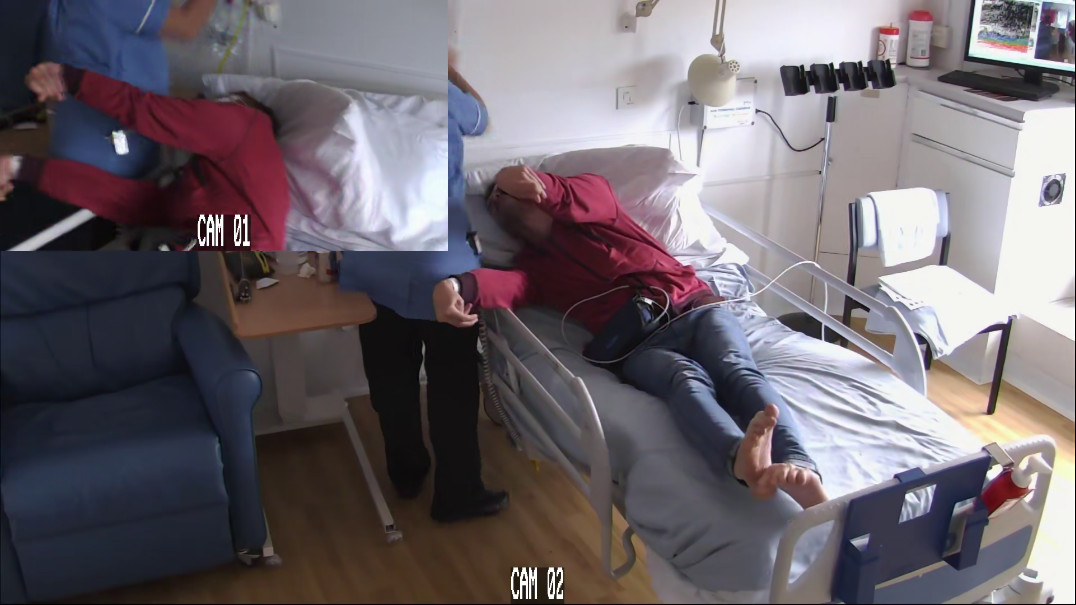
\includegraphics[trim=2mm 2mm 2mm 2mm, clip, width=\linewidth]{016_01}
  \end{subfigure}
  \begin{subfigure}{0.49\linewidth}
    
\includegraphics[trim=2mm 2mm 2mm 2mm, clip, width=\linewidth]{030_01_blurred}
  \end{subfigure}
  \caption[Examples of bilateral symmetric tonic arm extension]{
    Examples of bilateral symmetric tonic arm extension during \acfp*{FBTCS}.
    \acsp{FBTCS} have been associated with a higher risk of \acf*{SUDEP}.
  }
  \label{fig:decerebration}
\end{figure}

A seizure is defined as ``a transient occurrence of signs and/or symptoms due to abnormal excessive or synchronous neuronal activity in the brain'' \cite{fisher_epileptic_2005}.
In 2017, the \ac{ILAE} published a widely accepted classification of seizure types \cite{fisher_operational_2017}, which we follow in this work.
Grosso modo, seizures can be classified into three categories \cite{fisher_epileptic_2005} (\cref{fig:ilae_seizure_types}):
\begin{itemize}
  \item \textbf{\Acp{FOS}} start in one hemisphere of the brain. If they spread to the other hemisphere, \acp{FOS} become \acp{FBTCS}.
  \item \textbf{Generalized onset seizures} are characterized by an apparent onset in both hemispheres of the brain.
  \item \textbf{Unknown onset seizures} comprises seizures whose onset is unknown. They may be reclassified as \acp{FOS} or generalized as new information becomes available.
\end{itemize}

\begin{figure}
  \centering

  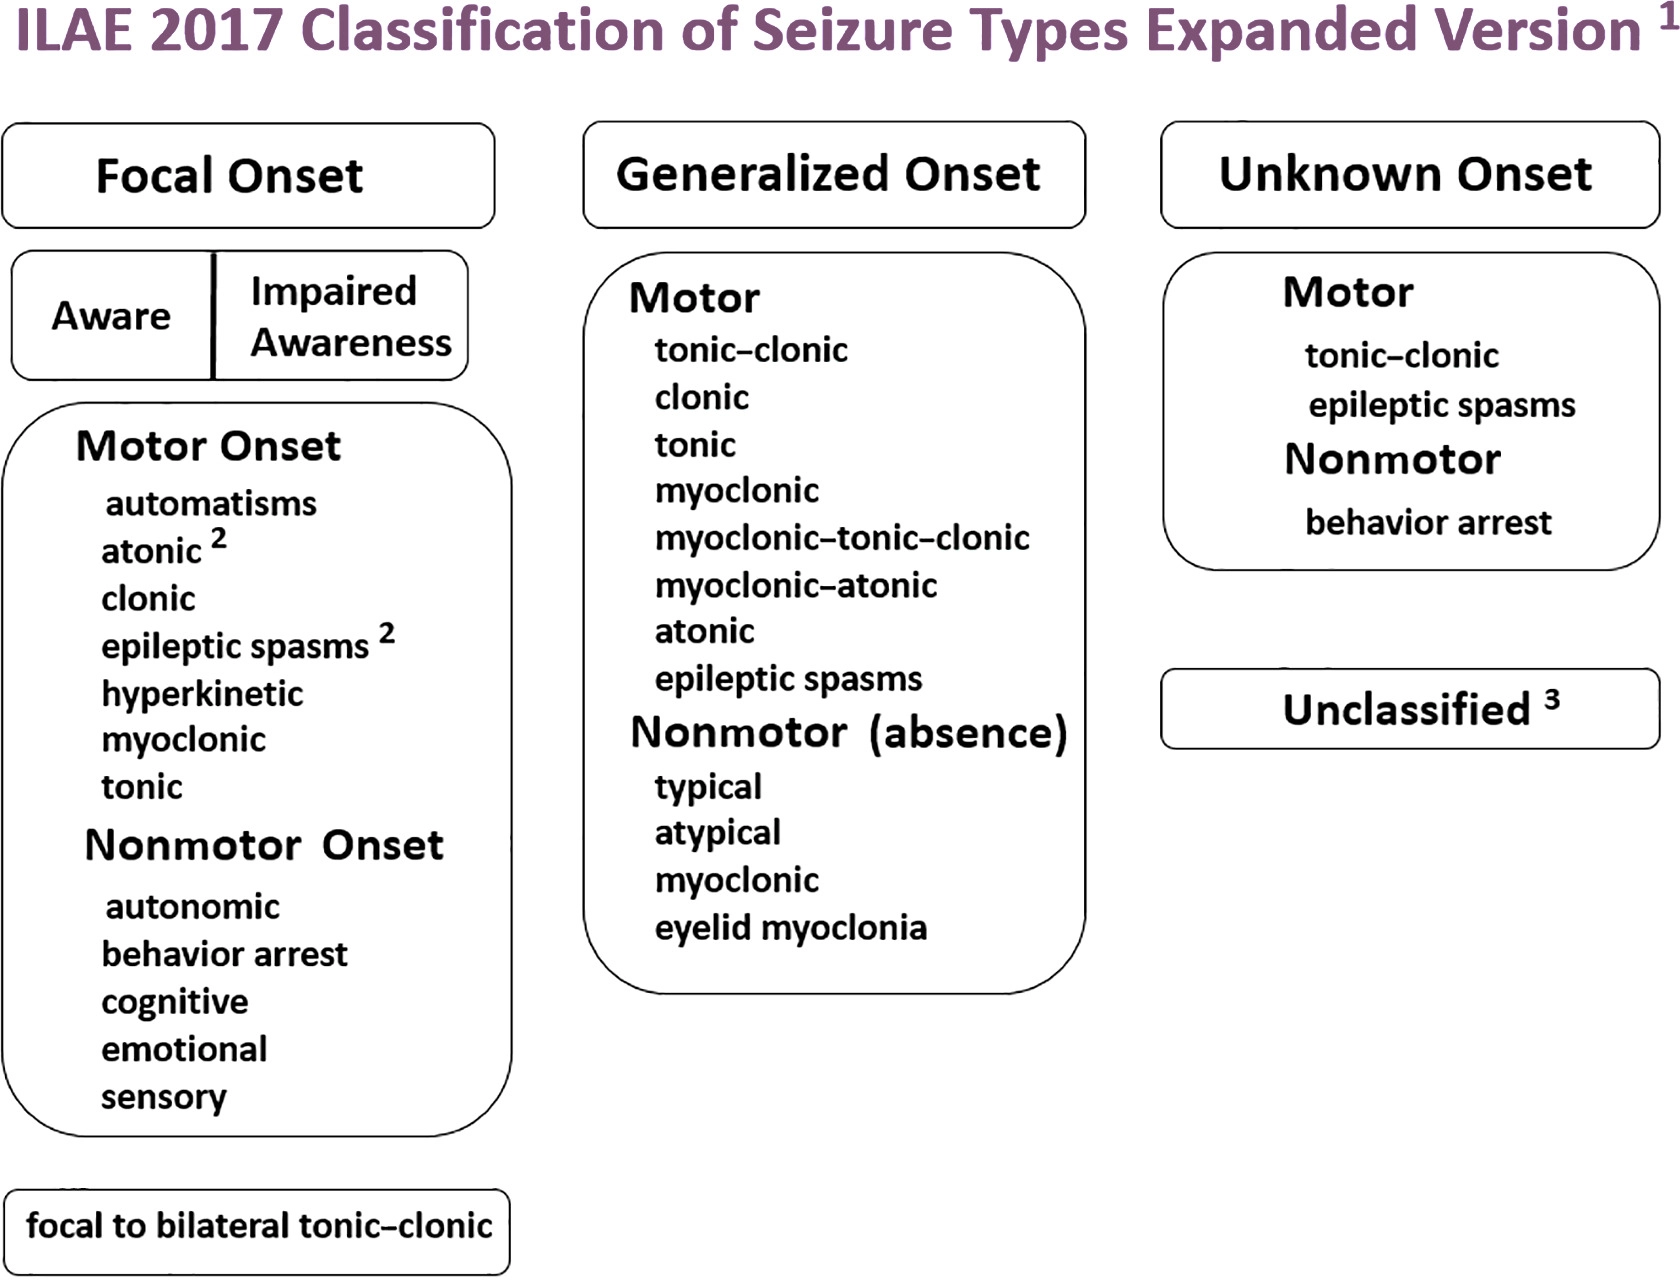
\includegraphics[width=0.8\linewidth]{ilae_seizure_classification}
  \caption[ILAE classification of seizure types]{
    \Acf*{ILAE} classification of seizure types (from \cite{fisher_operational_2017}).
  }
  \label{fig:ilae_seizure_types}
\end{figure}

Our work on automatic classification of seizure videos to aid in preventing sudden death is presented in \cref{chap:videos}.

\subsection{Presurgical evaluation}

\Ac{ASM} is normally used to treat epilepsy by decreasing the seizure frequency, but does not cure the underlying cause.
In roughly one third of the patients, \ac{ASM} does not adequately control seizures.
These patients are described as being medically refractory.
Half of the medically refractory epileptic patients have focal epilepsy, which may be treated by curative resective surgery.

The objective of resective epilepsy surgery is the complete resection or complete disconnection of the \ac{EZ}, which is defined as ``the area of cortex indispensable for the generation of clinical seizures'' \cite{rosenow_presurgical_2001}.
The surgery is performed if the \ac{EZ} can be definitely identified and is located in a part of the brain that may be removed without causing neurological, cognitive or neuropsychiatric deficit \cite{jobst_resective_2015}.

To locate the \ac{EZ}, \ac{EEG} and video-telemetry are acquired.
Analysis of these data may help lateralize or coarsely localize the \ac{EZ}.
Then, several preoperative imaging scans such as \ac{T1w} \ac{MRI} or \ac{T2w} \ac{FLAIR} \ac{MRI} are acquired to identify structural cerebral abnormalities, such as focal cortical dysplasia \cite{kabat_focal_2012}, hippocampal sclerosis \cite{thom_review_2014} or brain tumors.
If a structural lesion is found that is concordant with the results of \ac{EEG} and video-telemetry, the patient can be recommended for surgery \cite{duncan_brain_2016}.
However, 15 to 30\% of patients with focal epilepsy are \ac{MRI}-negative, meaning they have no distinct abnormalities visible from imaging or the abnormalities are discordant from video \ac{EEG} telemetry \cite{bien_characteristics_2009} (results are discordant when they suggest different \ac{EZ} localizations).
For example, an \ac{MRI} can show a lesion near the motor cortex, but \ac{EEG} shows abnormal activity in the occipital lobe.
In such cases, intracranial electrodes may be implanted to acquire \ac{iEEG} signals for precise localization of the \ac{EZ} (\cref{fig:electrodes}).

\begin{figure}[hbt!]
  \centering
  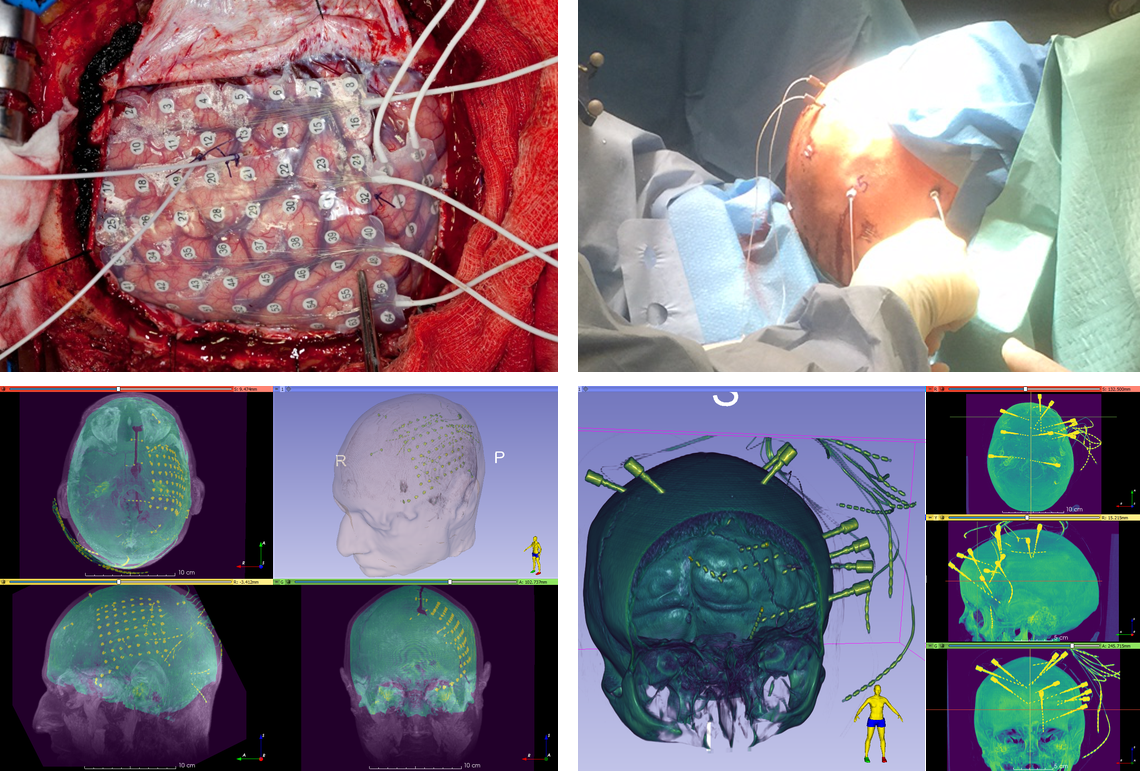
\includegraphics[width=\linewidth]{electrodes}
  \caption[Electrodes used for intracranial EEG]{
    Electrodes used for \acf{iEEG}.
    Left: subdural grid electrode;
    right: \acf{SEEG} depth electrodes.
    Top: intraoperative photos after electrode placement for each implantation procedure;
    bottom: volume renderings and \acfp{MIP} of post-implantation images.
    The skull is shown in green.
    The electrodes and cables are shown in yellow.
  }\label{fig:electrodes}
\end{figure}

The brain structures in which the electrodes are implanted are chosen by clinicians after interpretation of the aforementioned non-invasive data acquisition modalities, particularly seizure semiology, video-\ac{EEG} and \ac{MRI}.
However, there are significant variations in implantation strategies between centers, based on views regarding the relationship between semiological features and brain regions involved \cite{tufenkjian_seizure_2012}.
Therefore, tools to summarize findings across studies and highlight overall potential regions associated with a specific semiology may help standardize implantation approaches.

To determine an objective implantation plan for the \ac{iEEG} electrodes, we developed a data-driven tool that maps seizure semiologies to brain structures, using retrospective information from the literature (\cref{chap:svt}).

\subsection{Resective surgery}

If the \ac{iEEG} findings enable a definitive localization of the \ac{EZ}, surgery to resect the determined \ac{EZ} may be performed.
Currently, only 40\% to 70\% of patients with refractory focal epilepsy are seizure-free%
\footnote{In this context, ``seizure freedom'' refers to one year without seizures from the surgery.}
after surgery \cite{jobst_resective_2015}.
This is, in part, due to limitations identifying the \ac{EZ}.
Retrospective studies relating presurgical clinical features and resected brain structures to surgical outcome provide useful insight to guide \ac{EZ} resection \cite{jobst_resective_2015}.
To quantify resected structures, the resection cavity, which is mostly composed of \ac{CSF} (\cref{fig:cavities}), must be segmented on the postoperative \ac{MRI}.
A preoperative image with a corresponding brain parcellation can then be registered to the postoperative \ac{MRI} to identify resected structures.

Manual segmentation of brain resection cavities on 3D images is a time-consuming process requiring highly trained individuals, and a high inter-rater variability is usual \cite{havaei_brain_2017}.
A tool for automatic segmentation would facilitate and accelerate the research to better understand the relation between the clinical features and surgical outcomes.
% However, automatic techniques for cavity segmentation are challenging as other structures in the brain may look similar, such as the ventricles, cysts or oedemas (\cref{fig:}).
% Moreover, brain shift can happen during surgery, creating parts of the images that are also filled with \ac{CSF}.
Our work on automatic segmentation of brain resection cavities is presented in \cref{chap:resection}.


\newcommand{\plotcavities}[2]{
  \begin{subfigure}{0.8\linewidth}
    \includegraphics[trim=0 0 0 50, clip, width=\linewidth]{percentiles/#1}
    \caption{#2}
  \end{subfigure}
}

\begin{figure}
  \centering

  \plotcavities{p_050_0185_arrows}{Resection cavity in the temporal lobe}
  \plotcavities{p_075_1263_arrows}{Resection cavity in the frontal lobe}
  \plotcavities{p_025_0039_arrows}{Resection cavity in the parietal lobe}

  \caption[Examples of brain resection cavities after curative epilepsy surgery.]{
    Examples of brain resection cavities (marked with green arrows) after curative epilepsy surgery.
  }
  \label{fig:cavities}
\end{figure}

